\documentclass[tikz]{standalone}
\begin{document}
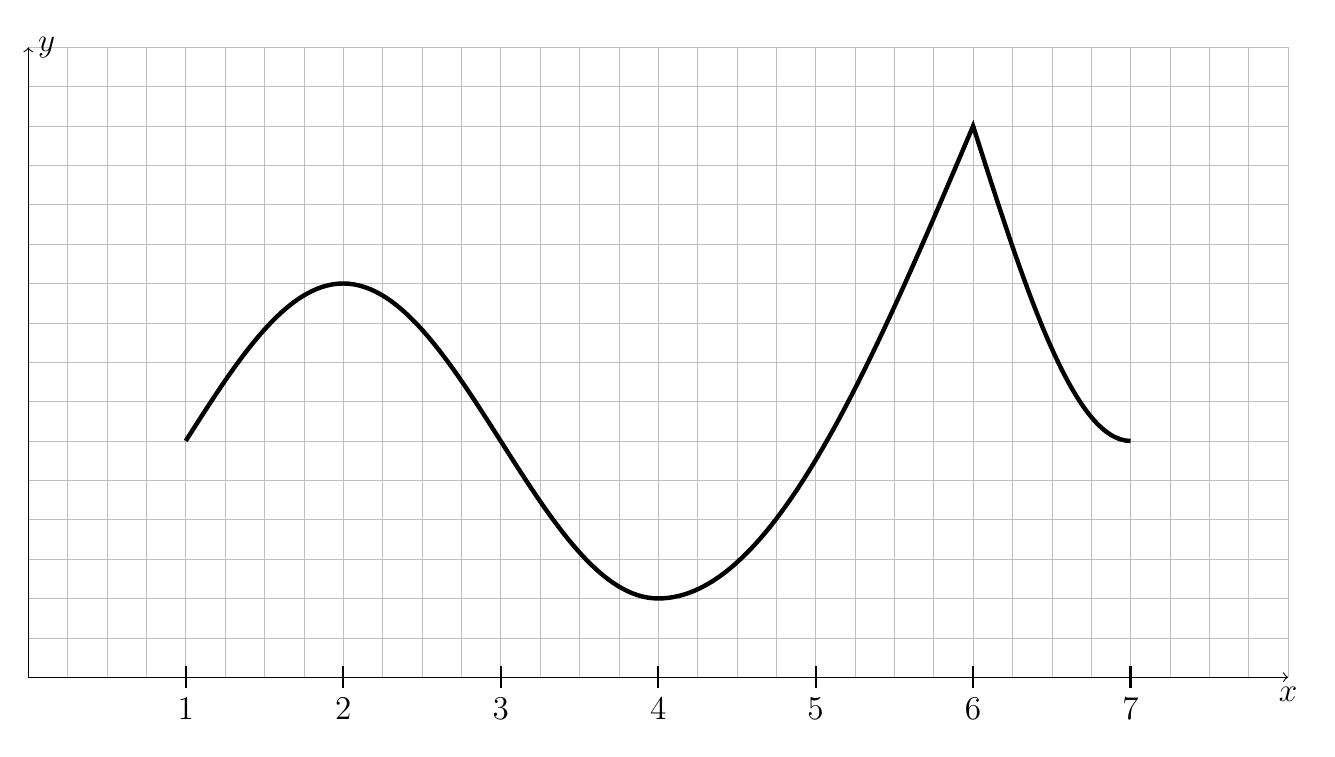
\begin{tikzpicture}[scale=2.0]
\tikzstyle{every node}=[font=\large]

\draw[white,fill=white] (0,0) rectangle (8,4);
 \draw[very thin,color=darkgray,step=1.0] (0,0) grid (8,4);
 \draw[very thin,color=lightgray,step=0.25] (0,0) grid (8,4);

\draw[->] (0,0) -- (8,0) node[below] {$x$};
\draw[->] (0,0) -- (0,4) node[right] {$y$};
     
% draw curve
\draw [ultra thick] 
(1,1.5) sin (2,2.5) cos (3,1.5) sin (4,0.5) cos (6,3.5) sin (7,1.5);


% tick marks
\foreach \x in {1,...,7} 
	\draw [thick] (\x cm,2pt) -- (\x cm,-2pt) node[below] {$\x$};
\end{tikzpicture}
\end{document}
